

\section{測定準備のためのコマンド}
\begin{itemize}

\item 接続しているdeviceの確認
\begin{screen}
\begin{verbatim}
$ nmcli device
\end{verbatim}
\end{screen}

\begin{screen}
\begin{verbatim}
$ nmcli con up enp0s31f6
\end{verbatim}
\end{screen}

\begin{screen}
\begin{verbatim}
$ setnew
$ setord
\end{verbatim}
\end{screen}

\item Pyrameのストップ・スタート
\begin{screen}
\begin{verbatim}
$ stoppy[systemctl stop pyrame]
$ startpy[systemctl start pyrame]
\end{verbatim}
\end{screen}


\item thresholdDACの値の設定\\
以下のコマンドの***に threshold DAC の値を代入する。
\begin{screen}
\begin{verbatim}
$ change_trigth.sh  /opt/calicoes/config/wagasci_config_dif1_chip1.txt ***
\end{verbatim}
\end{screen}



\item preampDACの値の設定\\
\begin{screen}
\begin{verbatim}
$ wgChangeConfig -c -r -f /opt/calicoes/config/wagasci_config_dif1_chip1.txt
 -m 3 -b 36 -v 53
\end{verbatim}
\end{screen}


\item InputDACの値の設定\\
\begin{screen}
\begin{verbatim}
$ wgChangeConfig -c -r -f /opt/calicoes/config/wagasci_config_dif1_chip1.txt 
-m 2 -b 36 -v 41
\end{verbatim}
\end{screen}

\end{itemize}

引数の意味は以下の表の通り。
\begin{table}[H]
\begin{center}
\caption{wgChangeConfig の引数}
\begin{tabular}{ccc} \hline
引数名 & 意味 & 備考 \\ \hline
m &  &  \\
b & チャンネル指定 & 36なら全チャンネルを、0-35ならそのchを意味する。 \\
v & DACの値 &  \\ 
\hline
\end{tabular}
\end{center}
\end{table}
なお、txtファイルのdif、chipの後の数字でそれぞれDIFとChipの番号を指定できる。\\

\newpage
\section{実際の測定の流れ}

\begin{enumerate}
\item GDCC/CCCの立ち上げ\\
LV\_GDCC/CCCをon (1.2Vぐらいから少しずつ上がり1.8〜1.9Vになる)

\item Low voltage (LV) の立ち上げ\\
LV\_IF をon (~0.54V)

\item xmlファイルの読み込み・Configure\\
ASUが1枚の場合と3枚の場合はそれぞれ、
\begin{screen}
\begin{verbatim}
$ load_config_file.sh /opt/calicoes/config/wagasci_config_1asu.xml[load]
$ load_config_file.sh /opt/calicoes/config/wagasci_config_3asu.xml[load3]
\end{verbatim}
\end{screen}
さらに、初期化、configureを行う。
\begin{screen}
\begin{verbatim}
$ init[initialize.sh]
$ conf[configure.sh]
\end{verbatim}
\end{screen}
この時点でLV\_IFの電圧が少し上昇する。[Ex.) 0.54 A $\to$ 0.58-0.61 A]\\

\textcolor{red}{これなんだろう?}
\begin{screen}
\begin{verbatim}
spill_setinfo.sh p 
spill_setinfo.sh a
spill_getinfo.sh
\end{verbatim}
\end{screen}

\item HVの立ち上げ\\
HVを入れる、3.5 V から出力し、徐々に(1 V ずつ)上げていく。0 V から始めないのは、微小なバイアス電圧をかけた段階で反対方向に電流が流れるのを防ぐため\textcolor{red}{?}。

\item spillの開始\\
internal spill を利用する場合は以下のコマンドを利用する。
\begin{screen}
\begin{verbatim}
$ spill_internal.sh
\end{verbatim}
\end{screen}
この時、GDCCの前面のLightが点滅する。なお、internal spillで送られる信号は周期 260 msec、パルス幅 5 msec の方形波である。\\

外部トリガーを使って測定を行う場合は、
\begin{screen}
\begin{verbatim}
$ spill_external.sh
\end{verbatim}
\end{screen}
を用いる。その際、写真の場所に信号を入れる。

\begin{figure}[H]
\begin{center}
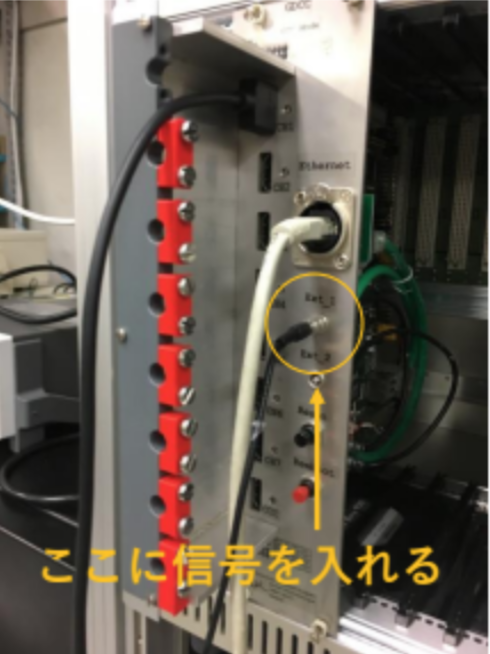
\includegraphics[width = 6.0cm, bb= 0 0 490 654]{external_trigger_input.png}
\end{center}
\caption{外部トリガーの入力端子}
\label{fig:}
\end{figure}

spillの設定を変更したいときは、/SiTCP/scriptの中のspill\_setinfo.shというコマンドを用いる。\\
※このコマンドがないときはAnalysis/bin/wgChangeConfigを使用。
\begin{screen}
\begin{verbatim}
$ wgChangeConfig -f CONFIG_FILE_NAME.txt
\end{verbatim}
\end{screen}
で同じように確認できるはず。これを使用すればconfigをこのコマンドのみで変更できる。

\item 測定の開始\\
以下のコマンドで測定のスタート、ストップができる。
\begin{screen}
\begin{verbatim}
$ start_run.sh ********* remove

$ stop_run.sh *********
\end{verbatim}
\end{screen}

\item 終了方法\\
測定前と逆の手順を行う。
\begin{itemize}
\item HVを消す
\item LV\_IFを消す
\item LV\_GDCC/CCCを消す
\end{itemize}

\item データを見る\\
rawデータをデコードする必要がある。
\begin{screen}
\begin{verbatim}
$ Decoder -f  /home/data/prototech/******/******.raw
\end{verbatim}
\end{screen}
これにより、/home/data/decode/ 以下に root ファイルが生成される(旧:/home/data/rootfile/)。\\
rootファイルができる場所を指定する (DIR\_NAME) には、デコードする際に
\begin{screen}
\begin{verbatim}
$ Decoder -f  /home/data/prototech/******/******.raw -o /PATH/TO/DIR_NAME
\end{verbatim}
\end{screen}
とする。\\

running中のデータを見るには、ls を用いる。

\end{enumerate}

\newpage
\section{環境変数の設定}

\subsection{環境変数の設定}
WAGASCI関連の環境変数はsetting\_wagasci.shに記述されている。

\begin{table}[H]
\begin{center}
\caption{setting\_wagasci.sh}
\begin{tabular}{ll} \hline
ディレクトリパス & 意味  \\ \hline
WAGASCI\_RAWDATADIR & raw dataが出力されるディレクトリ\\
WAGASCI\_DECODEDIR   & Decodeした~\_tree.rootの出力先のデフォルト\\
WAGASCI\_HISTDIR         & wgMakeHistでヒストグラムを生成した~\_hist.rootの出力先のデフォルト\\
WAGASCI\_RECONDIR     & wgReconで飛跡再構成した~\_recon.rootの出力先のデフォルト\\
WAGASCI\_XMLDATADIR & wgAnaHistで\_hist.rootを解析したxml fileの出力先のデフォルト\\
WAGASCI\_IMGDATADIR  & 諸々で図を生成した場合の出力先のデフォルト\\
WAGASCI\_LOGDIR         & コマンド実行時のログの出力先のデフォルト\\
WAGASCI\_MAINDIR       & Analysis ディレクトリへのパス\\
WAGASCI\_RUNCOMMANDDIR  & RunCommand ディレクトリへのパス\\
WAGASCI\_CALICOE       & /opt/calicoeディレクトリへのパス\\
WAGASCI\_CALIBDATADIR & Calibration結果をまとめているディレクトリへのパス\\
WAGASCI\_BSDDIR         & beam summary dataへのパス\\
WAGASCI\_DQDIR           & wgDQCheckで出力するデータクオリティ用のファイルへのパス\\
WAGASCI\_DQHISTORYDIR  & wgDQHistoryで出力するデータクオリティの結果を纏めたファイルの出力先 \\ \hline
\end{tabular}
\end{center}
\end{table}

\subsection{新しくディレクトリを作る場合}
\begin{enumerate}
\item ディレクトリの作成\\
もし対応するディレクトが存在しない場合,mkdirでディレクトリを作って

\item setting\_wagasci.sh の編集\\
そのディレクトリへの絶対パスをsetting\_wagasci.shに書き込み、
\begin{screen}
\begin{verbatim}
$ source setting_wagasci.sh
\end{verbatim}
\end{screen}
で設定を読み込む。
\item bash.rc の編集\\
環境設定はターミナル終了時に消えてしまうので、ターミナル起動時に自動で読み込みを行うために ~/.bashrcに
\begin{screen}
\begin{verbatim}
source /PATH/TO/setting_wagasci.sh
\end{verbatim}
\end{screen}
と書き込む。
\end{enumerate}

\newpage
\section{CCCとの接続}
\begin{itemize}
\item enp0s31f6のIPアドレスを適切なもの (192.168.10.2 / 255.255.255.0 など)  に設定する
(やりづらければ、nmtuiを使用する。)
\item nmcli deviceを実行したら接続されているデバイスが表示される
\item nmcli con up enp0s31f6で接続が行われる
\item systemctl restart NetworkManagerで接続の反映
\end{itemize}




\section{txtファイルの確認方法}

\begin{screen}
\begin{verbatim}
# cd Analysis
# make clean
# make
# ./bin/wgChangeConfig -f wagasci_config_dif1_chip1.txt

# /usr/local/src/wagasci_software/Analysis/bin/wgChangeConfig 
-f /opt/calicoes/config/wagasci_config_dif1_chip1.txt 
\end{verbatim}
\end{screen}




※binの中に入っている実行ファイルは
\begin{screen}
\begin{verbatim}
# ./bin/wgChangeConfig -h
\end{verbatim}
\end{screen}

のよう
にしてそれぞれヘルプが見れます。


\section{よくあるエラー}
\begin{itemize}
\item 急にconfigure.shがうまくいかなくなる。\\
→LVを付け直し、まずGDCC/CCCのLVをつけ1.2Aぐらいから上昇し、1.9Vぐらいまで上昇したことを確認してから、IFのLVをつける。(この作業は正確に)

\item IFのLVの値がおかしい\\
→フラットケーブル(ASU−IF)の接続が正しくない\\
→シルクに合わせる+全体的に中心になるようにセット\\
参考 ASU一つの場合
\begin{itemize}
\item 正常なとき\\
5 V をかけたときの電流値: 0.54 A $\to$ (configが通る) 0.58-0.61 A (CVに明かりが点灯)
\item 正常ではないとき\\
5 V をかけたときの電流値:2.2 A とか??(CCに明かりが点灯)
\end{itemize}
\end{itemize}

\newpage
\section{SPIROCについて}

\subsection{PADACについて}

1つはプリアンプの値が低すぎると安定してトリガーをかけるのが難しくなることに由来して
もう1つはプリアンプの値が低い場合、ゲインの線形性があまり良くなくなるということです。\\
後者はどの程度か見積もることが出来てませんが、DAC値が50程度なら問題なさそうです。
(30,40になるとどうなるかはわかりませんが。)\\
ここはどうtuningするかによって変わってくると思うので、うまく最適化してください。\\

For the Gain of each channel, the (voltage) gain is given by 15pF/Cfeedback (for the HG)\\
Cfeedback is $(63 - 6-\mathrm{bit\_Gain\_Code}) \times 25\ \mathrm{fF}$.\\
The Cfeedback can be tuned by 25 fF steps. However, there is a parasitic capacitance on the feedback, so the theoritical gain with 25 fF should be $15\ \mathrm{p} / 25\ \mathrm{f} = 600$ but real gain is lower. \\
→理論的には600ずつ変えられるが…


\subsection{4-bit threshold adjustmentについて}

個々のチャンネルに対してスレショルドの値を微調整しています。
これを使わない場合、chip内のスレショルドは一律の値になります。\\
single MPPC cardを使用するとどうなるかわかりませんが、
僕の知る限りでは個々のチャンネルの微調整をしなくとも
一律のp.e.にトリガーをかけることが出来ています。
single MPPCの方がarray型のものよりMPPCの個体差が小さいので
多分使わずともうまく調整できるのではないかと。

\subsection{Slow shaper fast shaper}

Basically, the fast shaper is used to generate the trigger and measure the time.\\
The slow shaper is intended to measure the charge (thus it is more filtered in order to increase the S/N ration). It is not intended to reduce pileup !


\subsection{thresholdDAC}
\subsubsection*{Q} 
Using 10-bit threshold DAC, The threshold voltage (Vth) is set as follows.
\[ V_{\mathrm{th}} = V_1 + (V_2 - V_1) \times \mathrm{DAC} /1024 \]

What is the value of V1 and V2?\\
I don't know the relationship between a threshold voltage and the value of 10-bit DAC.\\

\subsubsection*{A} 
Concerning the point 1, I join you a linearity measurement of the Threshold DAC :
\[ V_{\mathrm{out}} = A \times \mathrm{DAC\_Code} + B \]
You can see that the slope is $A = 2.22$ mV/DAC unit with an offset of about $B = 830$ mV.


\newpage
\section{その他のメモ}

\begin{figure}[H]
\begin{center}
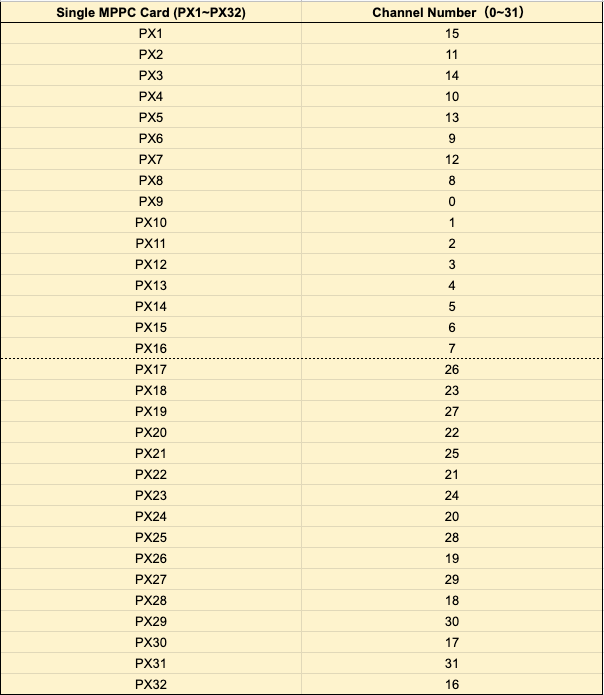
\includegraphics[width = 14.0cm, bb= 0 0 604 695]{single_mppc_board_id.png}
\end{center}
\caption{Single MPPC boardのPX-CH対応表}
\label{fig:}
\end{figure}

